\documentclass[linespread=1]{ctexart}
\usepackage[centering,b4j,body={683bp,34cm}]{geometry}

\usepackage{adfarrows}
\usepackage{adforn}
\usepackage{indentfirst}
\usepackage{fancybox}
\usepackage{graphicx}
\usepackage{makecell}
\usepackage{setspace}
\usepackage{textpos}
\usepackage{xcolor}

%\usepackage{tabularx}

\ctexset{autoindent=0}
%\ctexset{linespread=1}
%\ctexset{punct=quanjiao}
%\setlength{\parskip}{1ex}
\sloppy

\begin{document}
\thispagestyle{empty}
\begin{textblock*}{18\ccwd}(46\ccwd, 0\ccwd)
\Ovalbox{
\begin{minipage}[t]{18\ccwd}
\begin{center}
\doublespacing
\Large\hspace{2\ccwd}\rule{0pt}{23pt}本刊是计算机—激\\
光汉字编辑排版系统的\\
试排样张。\hspace*{4.8\ccwd}
\vspace{6pt}
\end{center}
\end{minipage}}
\end{textblock*}
\begin{minipage}[t]{46\ccwd}
\begin{center}
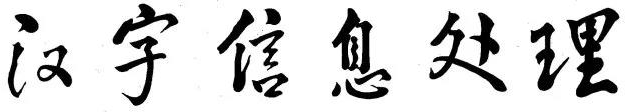
\includegraphics[width=40\ccwd]{wangxuan1979title.png}

\Large 报版样张\hspace{8\ccwd}1979 年 7 月 1 日\hspace*{2\ccwd}
\end{center}
\end{minipage}

\noindent\rule[5pt]{\textwidth}{1pt}\rule[5pt]{0pt}{10pt}

\ovalbox{
\begin{minipage}{64\ccwd}

\vspace{1em}
\begin{center}
\begin{minipage}{48\ccwd}
\Large\hspace{2\ccwd}由计算机总局主持,北京大学、新华社、山东省电子局、潍坊市电子局、\\[5pt]
潍坊电讯仪表厂、杭州五二二厂、天津红星厂等单位协作会战\\
\end{minipage}

\begin{minipage}{59\ccwd}
\noindent
\Huge\heiti 计算机—激光汉字编辑排版系统主体工程研制成功\linebreak
\end{minipage}
\vspace{-1em}
\end{center}
\end{minipage}}
\vspace{\ccwd}

\begin{textblock*}{5\ccwd}(60\ccwd,0.8\ccwd)
\begin{center}
\begin{minipage}{2\ccwd}
\LARGE%\showthe\baselineskip
%\show\baselinestretch
\begin{spacing}{1.43}
\textbf{汉字字模信息的存贮}
\end{spacing}
\end{minipage}
\end{center}
\end{textblock*}
\begin{textblock*}{21\ccwd}(44\ccwd,0\ccwd)
\begin{minipage}[t]{16\ccwd}
\setlength{\parindent}{2\ccwd}
实现汉字数字化存贮首先遇到的
难题是“三多”: 汉字的字数多,字\linebreak
体多,字号多。从印刷要求看,不仅
要收七千左右的字,还得有各种不同
的字体。从一般书报来说,字体就有
书版宋、报版宋、标题宋、仿宋、楷
体、黑体、长宋、扁宋、长黑、扁黑
等十多种;字号就有小六号、六号直
到初号,共十五种。

其次是文字质量问题,要保证字
型美观、笔锋明晰。这就要求字模的\linebreak
点阵密度高,报版字的密度应在一毫
米二十点以上,书版字的密度应在一
毫米二十五点以上。我们所做的分解
密度为一毫米二十九点,这就是说一
个五号字,要由一万个点组成。在上\linebreak
述条件下如以小字号 ( 小六号到三
号) 每种收七千字,大字号(小二号\linebreak
到特号) 每种收四千字,总共要有六
十五万个字头,这就需要二百亿位的
存贮量。

为了减少汉字字模的存贮量,日
本采用的办法是记录有笔划的黑段的
起始位置和长度,这样可节省近一半
的存贮量。日本经济新闻采用这种办
\end{minipage}

\vspace{1.5pt}
法,用几十亿位的大磁盘只存贮了十多万个汉字
字头。 这远远满足不了我们的要求。而且大容量
 磁盘体积大,价格较贵,存取速度慢。能否使汉
字信息大量压缩是整个系统的关键所在。日本电
气公司和日本京都大学在七十年代初就进行这一
方面的研制,他们研制的汉字信息压缩技术虽然
压缩倍数很高,但文字质量不好,因此未投入使
用。  

\hspace{2\ccwd}%
我们研制成功了一种确保文字质量的高倍数
汉字信息压缩技术,可使每个五号字的信息量下
降十二倍,即从一万位下降到平均八百位。这种
压缩方法还允许文字变倍,能变大变小并保证质
量。这样整体压缩倍数高达五百倍,只需四千万\linebreak
位的存贮量就能存下六十五万字头的全部信息。\\
在照排过程中,有一个微程序汉字点阵生成器把
汉字压缩信息高速复原成点阵。汉字信息压缩技
术的研制成功给汉字照排系统开辟了新的途径,\\
使得高速、廉价的先进汉字照排机成为可能。\\
\adfarrow{19}\adfarrow{19}\adfarrow{19}\adfarrow{19}\adfarrow{19}\adfarrow{19}\adfarrow{19}\adfarrow{19}%
\adfarrow{19}\adfarrow{19}\adfarrow{19}\adfarrow{19}\adfarrow{19}\adfarrow{19}\adfarrow{19}
\adforn{7} \adforn{7}
\end{textblock*}
\begin{textblock*}{1\ccwd}(43\ccwd,7.4\ccwd)
  \begin{center}
  \adforn{7} \adforn{7}
\adfarrow{21} \adfarrow{21} \adfarrow{21} \adfarrow{21} \adfarrow{21} \adfarrow{21} \adfarrow{21} \adfarrow{21}
\adfarrow{21} \adfarrow{21} \adfarrow{21} \adfarrow{21} \adfarrow{21} \adfarrow{21} \adfarrow{21} \adfarrow{21}
\adfarrow{21} \adfarrow{21} \adfarrow{21} \adfarrow{21} \adfarrow{21} \adfarrow{21} \adfarrow{21} \adfarrow{21}
\adfarrow{21} \adfarrow{21} \adfarrow{21} \adfarrow{21} \adfarrow{21} \adfarrow{21} \adfarrow{21} \adfarrow{21}
\adfarrow{21} \adfarrow{21} \adfarrow{20}
  \end{center}
\end{textblock*}
%\begin{textblock*}{21\ccwd}(44\ccwd,7.4\ccwd)

\begin{textblock*}{43\ccwd}(0\ccwd,1.7\ccwd)
\hspace*{3\ccwd}\begin{minipage}{37\ccwd}\LARGE\textbf{汉字编辑排版系统的工作流程和软件}\linebreak\end{minipage}
\end{textblock*}
\vspace{4.39\ccwd}
\begin{minipage}[t]{10\ccwd}
\hspace{2\ccwd}%
{\heiti 一、汉字怎样进入计算机}\hspace{\ccwd}本系统将采用
两种汉字键盘。一种是
大键盘,共四百键,每\linebreak
键九个字,可以脱机也
可以联机。当联机使用
时,每个键盘有一台汉
字显示器,每击一键产
生十四位代码直接进入\linebreak
计算机,并立即在显示
器上显出这一汉字字
形。另一种是中键盘,\,
共二百五十六键,每键
代表两个或三个字符\linebreak
\hspace*{2pt}(整字或组字部件),\;
每个汉字由若干字符组
成。输入一个汉字实际
平均按键不超过三键。\\
\hspace*{2\ccwd}%
{\heiti 二、输出供校对用的小样}\hspace{\ccwd}输入计算机的
文章经软件处理后在汉
字印字机上输出小样,\\
小样的汉字文字质量不
高,只供校对修改用。\\
\hspace*{2\ccwd}%
{\heiti 三、通过汉字显示
器联机修改文章}\hspace{\ccwd}校对
人员可通过显示器修改
文章。键盘上设有几十
个功能键,可以方便地
\end{minipage}%
\hspace{\ccwd}%
\begin{minipage}[t]{10\ccwd}
增、删、改,或把文章
的某一段移到另一段中
去,修改后的结果立即
在显示器上显示出来。\\
有十台汉字显示器可以
供十个校对人员同时使
用。\\
\hspace*{2\ccwd}%
{\heiti 四、通过版面显示
器作版面设计}\hspace{\ccwd}版面显
示器能显示相当于一版
参考消息的版面情况,\\
编辑人员可以打入修改
版面设计的命令,在软
\end{minipage}%
\hspace{\ccwd}%
\begin{minipage}[t]{10\ccwd}
件控制下很快在显示器
上显示出修改的情况,\\
一直到编辑人员满意为
止。\\
\hspace*{2\ccwd}%
{\heiti 五、软件把输入的
文章组成版面,形成照
排信息,控制激光照排
机工作}\hspace{\ccwd}软件分析输入
的排版要求,确定每个
汉字在版面上的位置形
成照排信息,照排控制
器按照排信息从字模存
贮器中取出所需的汉字
\end{minipage}%
\hspace{\ccwd}%
\begin{minipage}[t]{10\ccwd}
字模压缩信息,微程序
汉字点阵生成器再把压
缩信息复原成汉字点
阵,提供给光调制器,\\ 
控制激光扫描打点或不
打点,在底片上形成所
需要的版面。\\
\hspace*{2\ccwd}%
上述全部工作都是
在软件控制下进行的,\\
整个软件系统包括分时
操作系统、排版编辑程
序、命令处理程序、终
端程序等。
\end{minipage}

\begin{textblock*}{43\ccwd}(0\ccwd,0.5\ccwd)
\begin{minipage}{43\ccwd}
{\hfill \adforn{7} \adforn{7}
\adforn{65}\adforn{65}\adforn{65}\adforn{65}\adforn{65}\adforn{65}\adforn{65}\adforn{65}%
\adforn{65}\adforn{65}\adforn{65}\adforn{65}\adforn{65}\adforn{65}\adforn{65}\adforn{65}%
\adforn{65}\adforn{65}\adforn{65}\adforn{65}\adforn{65}\adforn{65}\adforn{65}\adforn{65}
  \adforn{7} \adforn{7} \hfill }
\end{minipage}
\end{textblock*}
\begin{textblock*}{32\ccwd}(11\ccwd,-14.17\ccwd)
\begin{minipage}[t]{16\ccwd}
\setlength{\parindent}{2\ccwd}
本系统的输出设备为滚筒式激光
照排机。它利用激光束在底片上扫描
打点,将点阵化的汉字按版面要求排
出,排版幅面相当于两版《参考消息》
的版面。排出一版所需的时间为一分
四十秒。扫描线密度为每毫米二十九
线。

滚筒式激光照排机的激光车上有
四支激光管发出的四束光分别通过四
个光调制器,再分别由四个聚光物镜
会聚在四支光纤维端面上。通过光纤
维的光由横移拖板上的物镜会聚在底
\end{minipage}%
\hspace{\ccwd}%
\begin{minipage}[t]{15\ccwd}
片上。在排版时主马达带动滚筒以
均匀的速度转动。横移拖板以均匀
的速度移动。使扫描头在底片上产
生螺旋形的扫描线,底片旋转一\linebreak
周。横移拖板带动扫描头在底片上
横向移过四条扫描线的宽度。照排
控制器按编辑排版的要求,将汉字
点阵信息以四行并行输出的方式,\\
用四路信号分别控制四个光调制器
按文字点阵使光束打开或关上,这
样就通过扫描头在底片上打点扫描
排出版面。
\end{minipage}%
\end{textblock*}
\begin{textblock*}{32\ccwd}(11\ccwd,-17\ccwd)
{\hspace*{3\ccwd}}\begin{minipage}[t]{26\ccwd}
\LARGE\heiti 滚筒式激光照排机的工作原理\linebreak
\end{minipage}%
\end{textblock*}

\begin{textblock*}{32\ccwd}(0\ccwd,1.4\ccwd) %FIXME
\begin{center}
\begin{minipage}[t]{27\ccwd}
{\LARGE \textbf{第四代 排字 机}}\linebreak
\vspace{-1\ccwd}
\begin{center}
{\heiti 激光和计算机的结合给排版系统和信息处理带来新的突破}
\end{center}
\end{minipage}%
\end{center}
\end{textblock*}
\vspace{7.43\ccwd}

\begin{textblock*}{44\ccwd}(0pt,0pt)
\begin{minipage}[t]{10\ccwd}
\setlength{\parindent}{2\ccwd}
一九五八年美国发
明了光机式西文照相排
字机,在计算机控制下
依靠光学和机械方法选
取字模,逐字照相形成
版面,这称为第二代排
字机,六十年代在美国
大量生产。由于汉字字
数很多,照排技术要求
更复杂得多,所以直到
七〇年左右,日本才研
制成功第二代汉字排字
机,目前已经开始推广
使用。一九六五年西德
研制成功阴极射线管输
出的第三代排字机,各
种字模以数字化二进位
的形式存放在计算机的
外存贮器——磁盘中,
\end{minipage}%
\hspace{\ccwd}%
\begin{minipage}[t]{10\ccwd}
用扫描打点的方式在阴
极射线管上显示出高质
量的文字后照相。三代
机的速度可以比二代机
快十倍,适用范围广,\\
七十年代已在美国和西
德大量投产。日本引进
西德和美国的技术于一
九七五年初步研制成第
三代汉字排字机,一九
七八年已有少数几台在
使用,估计今后几年内
将逐步成熟和普及,三
代机对底片要求高,对
所使用的阴极射线管分
因率也要求很高,这些
困难在我国目前的技术
条件下不易很快解决。

\setlength{\parindent}{2\ccwd}
第四代排字机采用
\end{minipage}%
\hspace{\ccwd}%
\begin{minipage}[t]{10\ccwd}
激光技术,用激光束在
底片上扫描打点形成版
面。由于激光很强,普
通底片便能感光,还可
用转印的方式在普通纸
上印出逼真的大样。更
有意义的是用三到五瓦
的强激光束直接打到版
材上就能形成凹凸版
面,免除了照相制版一
大套工序,称为激光直
接雕版,是今后的发\linebreak
展方向。 目前世界上只
有一家公司开始少量生
产第四代西文排字机。\\
日本正在研制第四代汉
字排字机,但尚未成
功。这里有一系列的困
难需要克服,例如字模
\end{minipage}%
\end{textblock*}

\begin{textblock*}{12\ccwd}(33\ccwd,-6.0\ccwd)
\begin{minipage}[t]{10\ccwd}
存贮问题、文字变倍问
题、激光只能逐线扫描
不能逐字扫描的问题,\\
等等。我们采取了一系
列特别的方法,圆满地
解决了所有困难。这标
志着我国计算机编辑排
版系统和汉字信息处理
技术达到了一个新的水
平。
\end{minipage}%
\end{textblock*}

\begin{textblock*}{32\ccwd}(33\ccwd,6.0\ccwd)
\begin{center}
\begin{tabular}{|c|c|l|l|}
\hline
\multicolumn{2}{|c|}{\heiti 名\rule{5\ccwd}{0pt}称}  & \rule{0pt}{18pt}{\heiti 研制成功的年代和国家} & \multicolumn{1}{c|}{\heiti 特\rule{5\ccwd}{0pt}点} \\[8pt]
\hline
\rule{0pt}{15pt}第一代 & 手动照排机 & 西文:一九四九年美国 & 效率很低,改版困难 \\[6pt]

第二代 & 光\hfill 机\hfill 式 & \makecell{西文:一九五八年美国\\汉字:一九六九年日本} &
 \makecell[l]{机械动作多,速度低\\适用面窄,不易维修} \\[13pt]

第三代 & 阴极射线管 & \makecell{西文:一九六五年西德\\汉字:一九七五年日本} &
 \makecell[l]{速度快,对底片要求\\高,不能出大样} \\[13pt]

第四代 & 激\hfill 光\hfill 扫\hfill 描 & \makecell[l]{西文:一九七六年英国\\汉字:日本正在研制} &
 \makecell[l]{速度快,适用面广,\\还能直接雕版} \\[11pt]
\hline
\end{tabular}

\vspace{3pt}
\texttt{{\color{lightgray}github.com/chenshuo/typeset}\hfill https://wangxuan.pku.edu.cn/{}}
\end{center}
\end{textblock*}

\end{document}
